\documentclass[../main.tex]{subfiles}

\graphicspath{{../images/}}

\usepackage[noend]{algpseudocode} % for pseudocode
\usepackage[plain]{algorithm} % float environment for algorithms
% preferred pseudocode style
\algrenewcommand{\algorithmicprocedure}{}
\algrenewcommand{\algorithmicthen}{}

% ``do { ... } while (cond)''
\algdef{SE}[DOWHILE]{Do}{doWhile}{\algorithmicdo}[1]{\algorithmicwhile\ #1}%

% ``for (x in y ... z)''
\newcommand{\ForRange}[3]{\For{#1 \textbf{in} #2 \ \ldots \ #3}}

\begin{document}
\pagestyle{fancy}
\chead{Module 7}
\rhead{Junseo Shin}
\lhead{CSE 4059}


\renewcommand{\thefigure}{\arabic{figure}}
\section*{Text Histogram}

\subsection*{Questions}

\begin{enumerate}
    \item Using shared memory on the intermediate privatized historgrams reduces the latency of 
    accessing locations especially when it is heavily contended i.e. when multiple threads have
    the same ASCII character. This will improve the throughput of the atomic operations with faster
    memory access. 

    \item Nsys Compute Profiler:
    \begin{figure}[ht]
        \centering
        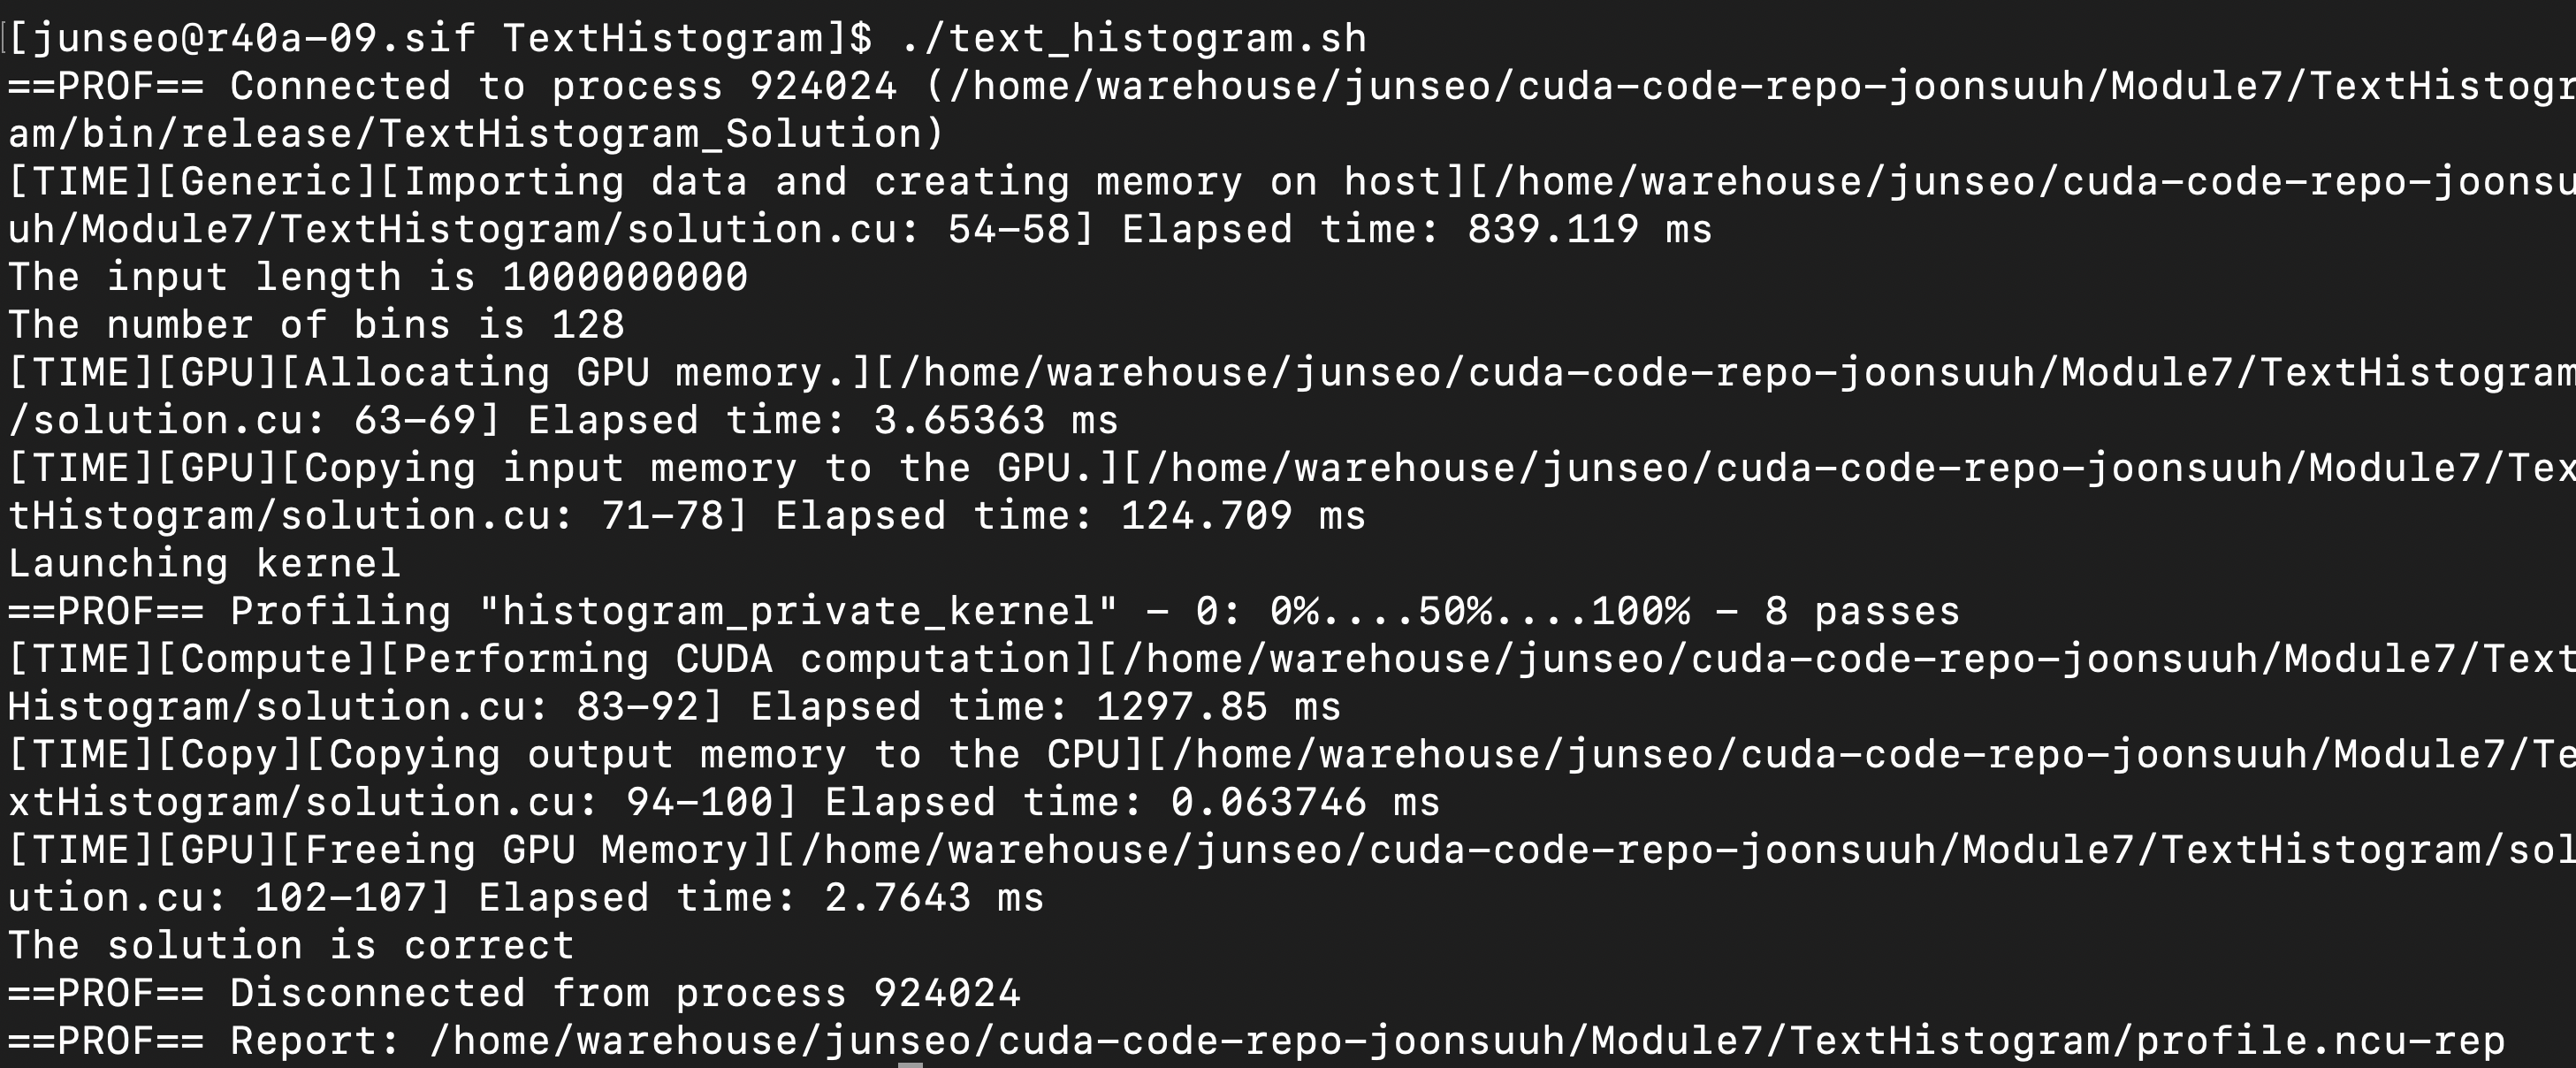
\includegraphics[width=0.8\textwidth]{texthistogram-prof.png}
        \caption{Nsys Compute Profiler}
        \label{fig:texthistogram-prof}
        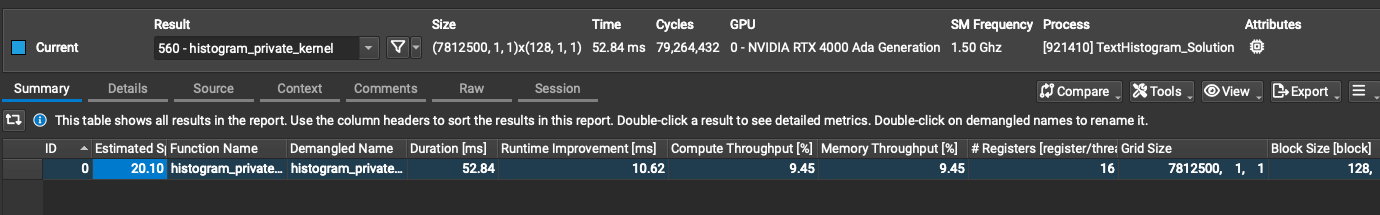
\includegraphics[width=0.8\textwidth]{histogram-ncu.png}
        \caption{Ncu Profiler}
        \label{fig:histogram-ncu}
    \end{figure}
    Although the profiler shows that we have an achieved occupancy of $88.72\%$, the GPU SOL
    throughput shows us the peak sustained rate was less than $10\%$. This is probably due to the
    large overhead of privatization where the number of launched thread blocks is smaller than the
    number that can be simultaneously launched by the GPU leading to serialization. This could
    be improved with thread coarsening or having a thread go through multiple input characters.

    \item In the histogram adding step \texttt{atomicAdd(\&bins\_s[input[tid]], 1u);} has to
    read from global memory once per thread, so for an input length $N$ we have $N$ global memory
    reads.

    \item In the for loop we are incrementing by \texttt{blockDim.x} up to the number of bins, so
    there are $\texttt{numBins} * \textrm{number of blocks}$ global memory writes.

    \item In shared memory, we have $N$ atomic operations since it happens along the histogram
    adding step in the privatized part. In global memory which is the final lines of code on the
    kernel function, we have \texttt{numBins} $\times$ \texttt{numBlocks} atomic operations.

    \item For a histogram without privatization or shared memory, there would be $N$ atomic
    operations performed in global memory. This ratio of the speed up compared to the privatized
    version is
    \begin{align*}
        N &: \texttt{numBins} \times \texttt{numBlocks} \\
        N &: \texttt{numBins} \times \frac{N}{\texttt{threads per block}} \\
        1 &: \frac{\texttt{numBins}}{\texttt{threads per block}}
    \end{align*}
    So for $128$ bins and $1024$ threads per block, the speed up is $1 : 128 / 1024 = 8 : 1$.
    


\end{enumerate}

\newpage
\subsection*{OUPUT}
\begin{figure*}[ht]
    \centering
    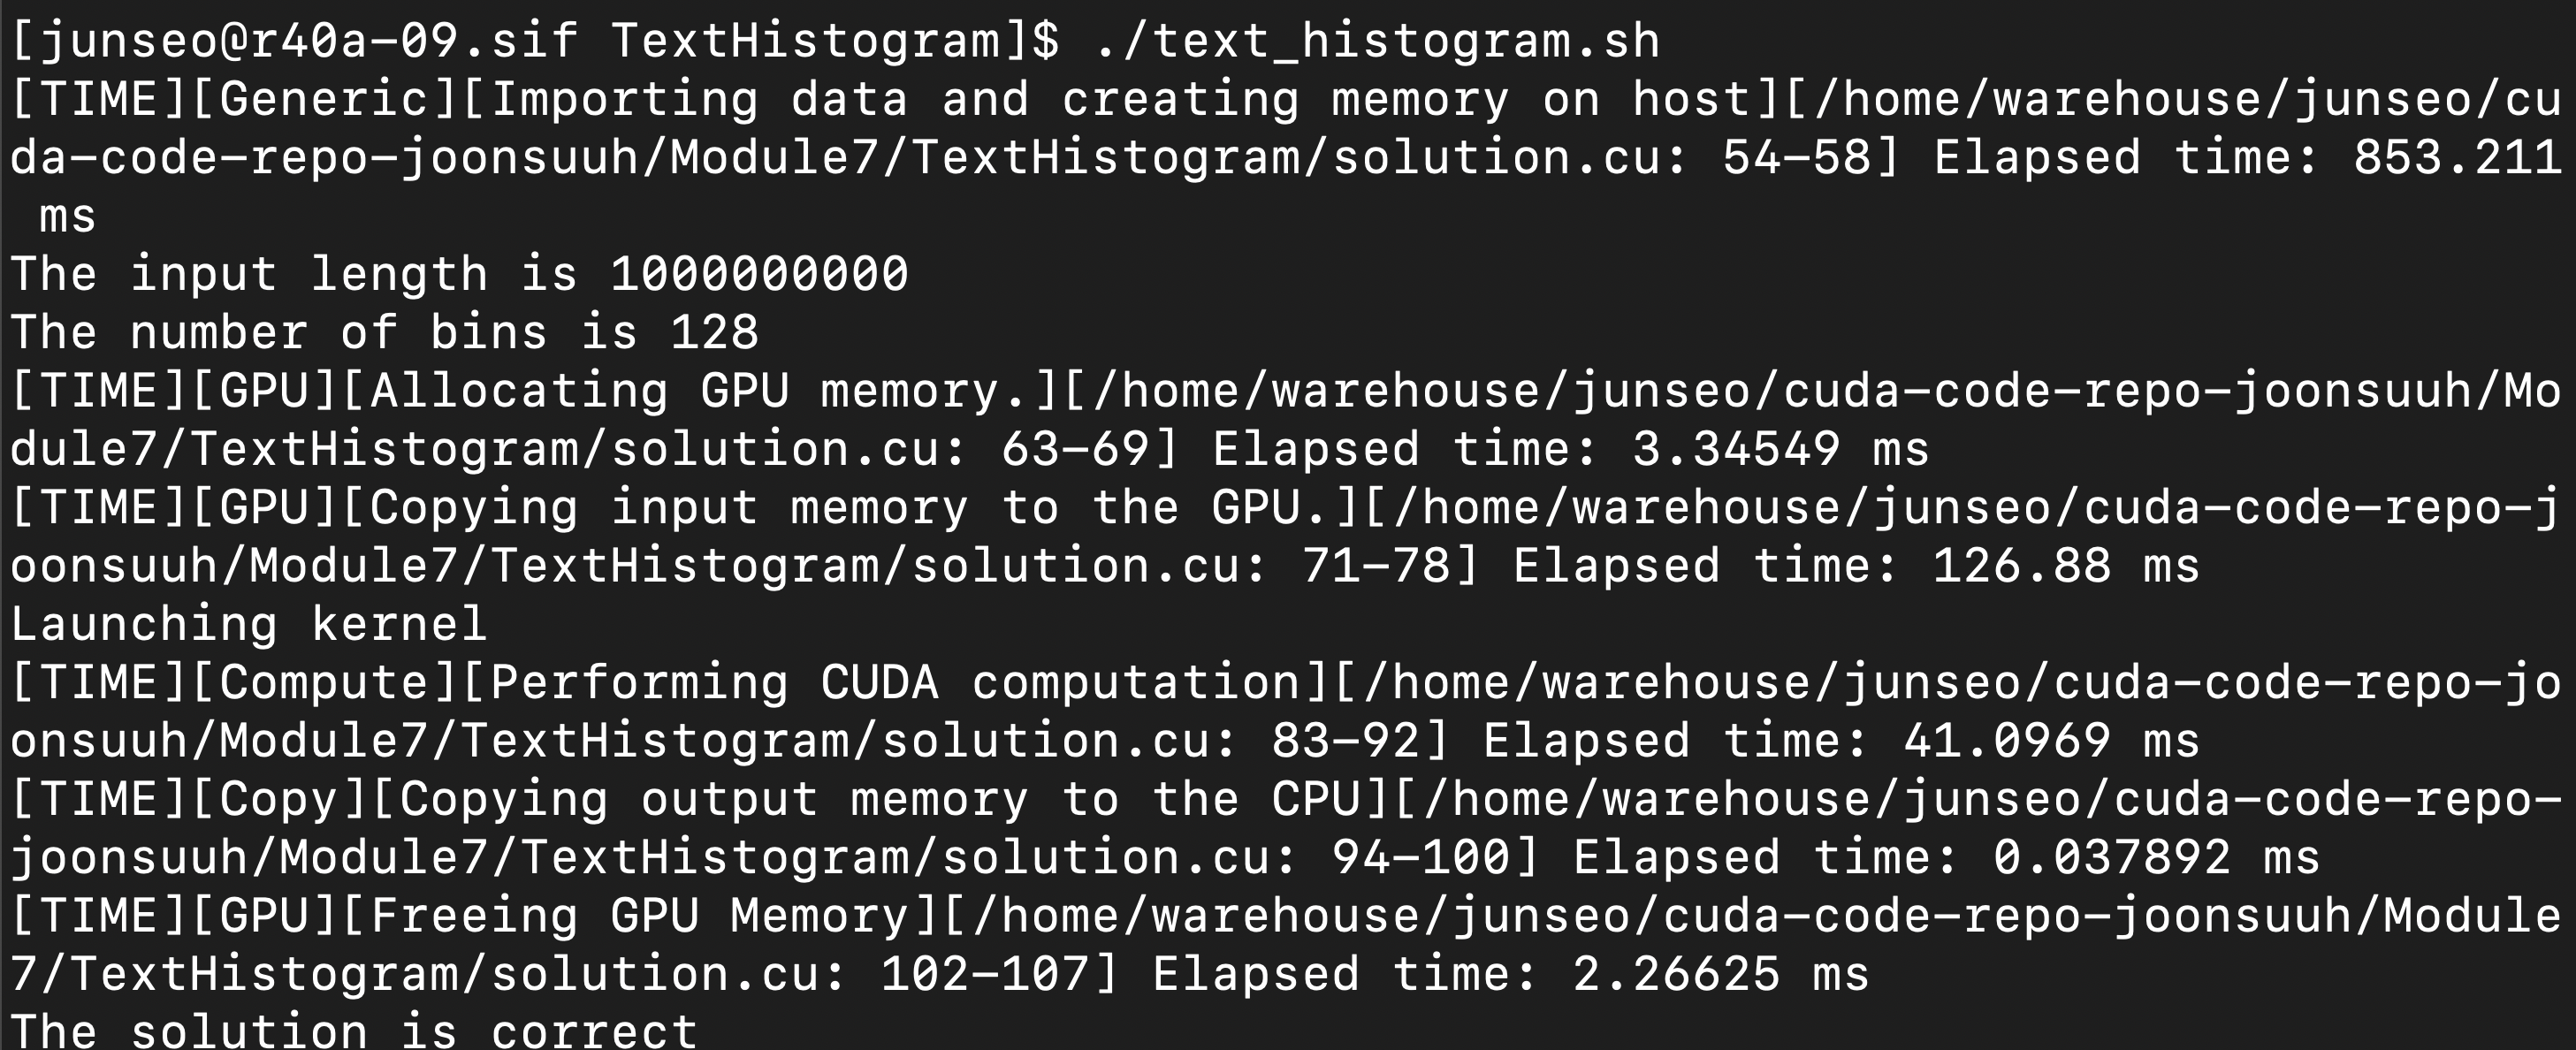
\includegraphics[width=0.8\textwidth]{texthistogram.png}
    \caption{Dataset 14 success ouput}
    \label{fig:texthistogram}
\end{figure*}

\end{document} 